\chapter{总结与展望}
\section{工作总结}
在本项工作中,我们主要探讨了经典的间断伽辽金方法,主要是以内罚形式实现。在此基础上,我们将间断有限元和时空方法结合,基于热方程以及NS方程介绍其理论,并完成了相关的数值算例,证明了经典算法的可行性。
在此基础上我们从另外一个角度看待了有限元类方法,将深度学习的方法和DG方法相结合,在现有处理弱形式方程的基础上进行改进,提出了新的思路,并通过了相关的数值算例,证明了其方法的可靠性。

DGNet其实本质上是一种自适应的想法。在一些没有出现复杂解的情况下其实没必要将网络拆开。
这也就是为什么间断有限元在求解有间断解等问题上展现出优势,而在一般的问题上用间断方法其实增加了计算量。
也就是说当网络的非线性性足够去拟合一个方程的解的时候,没有必要将网络拆分成小的网络。
因为可以看到为了小网络之间的耦合,我们添加了两个惩罚项在损失函数中作为约束,这其实增加了优化的难度。因此当网络很大,比如单个拥有4层50个神经元的隐藏层网络
不足以拟合某个,例如有高频振荡,或者间断解的问题时,可以采用DGNet的方法。    
\section{研究展望}
首先值的说明的第一是实验代码还有很大的优化空间,现在的训练速度还不够快,只是对于一些基本问题方案体现了其合理性。
第二DG方法主要的优势在与间断跳跃解,在局部存在奇点的情况。这些情况在本项工作中还没有体现,而仅仅完成了初步的实验。因此对于实验还有很多需要完善的地方,无论是和经典的PINN等方法的精度和训练速度对比。
第三关于将Split DG Net应用到时空有限元方法上应该是很自然的,但是这部分实验还未来得及实践。

但我仍然认为这是一个非常值的继续研究的方法,尤其是在完成在时空有限元方法上的实践之后,很自然的可以应用到1.动边界的处理上面,在工业上例如半导体制造中的薄膜沉积的仿真上;2.区域分解,在不同区域进行不同的离散化之后可以实现微观和宏观部分的耦合,是多尺度所关心的问题。

还有一些思路还未来得及尝试,在未来工作中可以再去具体实现:
\subsection*{数据监督}
其实,深度学习很大一部分优势还在于数据。因此当我们拥有数据之后,可以让优化变得更加简单。在上述的工作中,最终的约束损失函数中有四项,这对于没有数据只进行优化的深度学习任务来说是很困难的。
但是当我们拥有数据后,我们不仅在局部可以拆分成拥有边界信息的小块,从而进行训练,而且机理也可以部分未知,实现反问题的求解。
当局部数据给定之后,由于单元上网络的独立,可以通过固定除了单元以及单元邻居外的网络的参数,仅仅进行局部的参数调整来加快训练速度。

\subsection*{图神经网络}
图神经网络近些年也展现出它强大的威力,尤其是在处理图形数据的时候。然而对于三角化之后的离散区域,我们很容易发现,三角单元之间的关系就是图状结构,并且有封闭的性质,如图2维可以抽象为:


\begin{figure}[H] 
    \centering  
    \begin{subfigure}{0.4\textwidth}  
        \centering  
        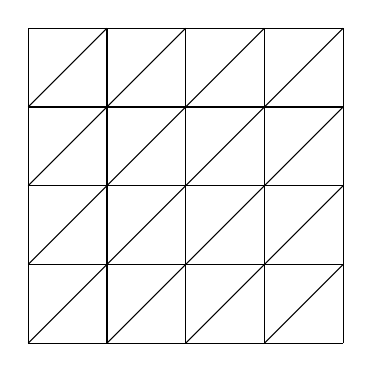
\begin{tikzpicture}  
            \draw (0,0) -- (4,0);  
            \draw (0,1) -- (4,1);  
            \draw (0,2) -- (4,2);  
            \draw (0,3) -- (4,3);  
            \draw (0,4) -- (4,4);  
            \draw (0,0) -- (0,4);  
            \draw (1,0) -- (1,4);  
            \draw (2,0) -- (2,4);  
            \draw (3,0) -- (3,4);  
            \draw (4,0) -- (4,4);  
            \foreach \y in {0,1,2,3}  
            {  
                \draw (\y,0) -- (4,4-\y);
            }  
            \foreach \y in {1,2,3}  
            {  
                \draw (0,\y) -- (4-\y,4);   
            }  
        \end{tikzpicture}  
        \caption{Triangluation}  
    \end{subfigure}  
    \begin{subfigure}{0.4\textwidth}  
        \centering  
        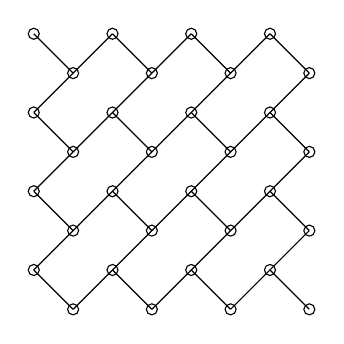
\begin{tikzpicture}  
            \foreach \y in {0,2,4,6}
            {\foreach \x in {0,1,2,3}
            {
                \draw (\x ,\y * 0.5 + 0.5) circle (2pt);
                \draw (\x + 0.5,\y * 0.5) circle (2pt);
            }}
            \foreach \x in {0,1,2}
            {
                \draw (0, \x + 0.5) -- (3 - \x,3.5);
                \draw (0.5 + \x, 0) -- (3.5, 3 - \x);
            }
            \foreach \x in {0,1,2,3}
            \foreach \y in {0,1,2,3}
            {
                \draw (\x, \y + 0.5) -- (\x+0.5,\y);
            }
        \end{tikzpicture}  
        \caption{Graph of cells}  
    \end{subfigure}  
\end{figure}  

三维可以表示为:

\begin{figure}[H]
    \centering  
    \begin{subfigure}{0.5\textwidth}  
        \centering  
        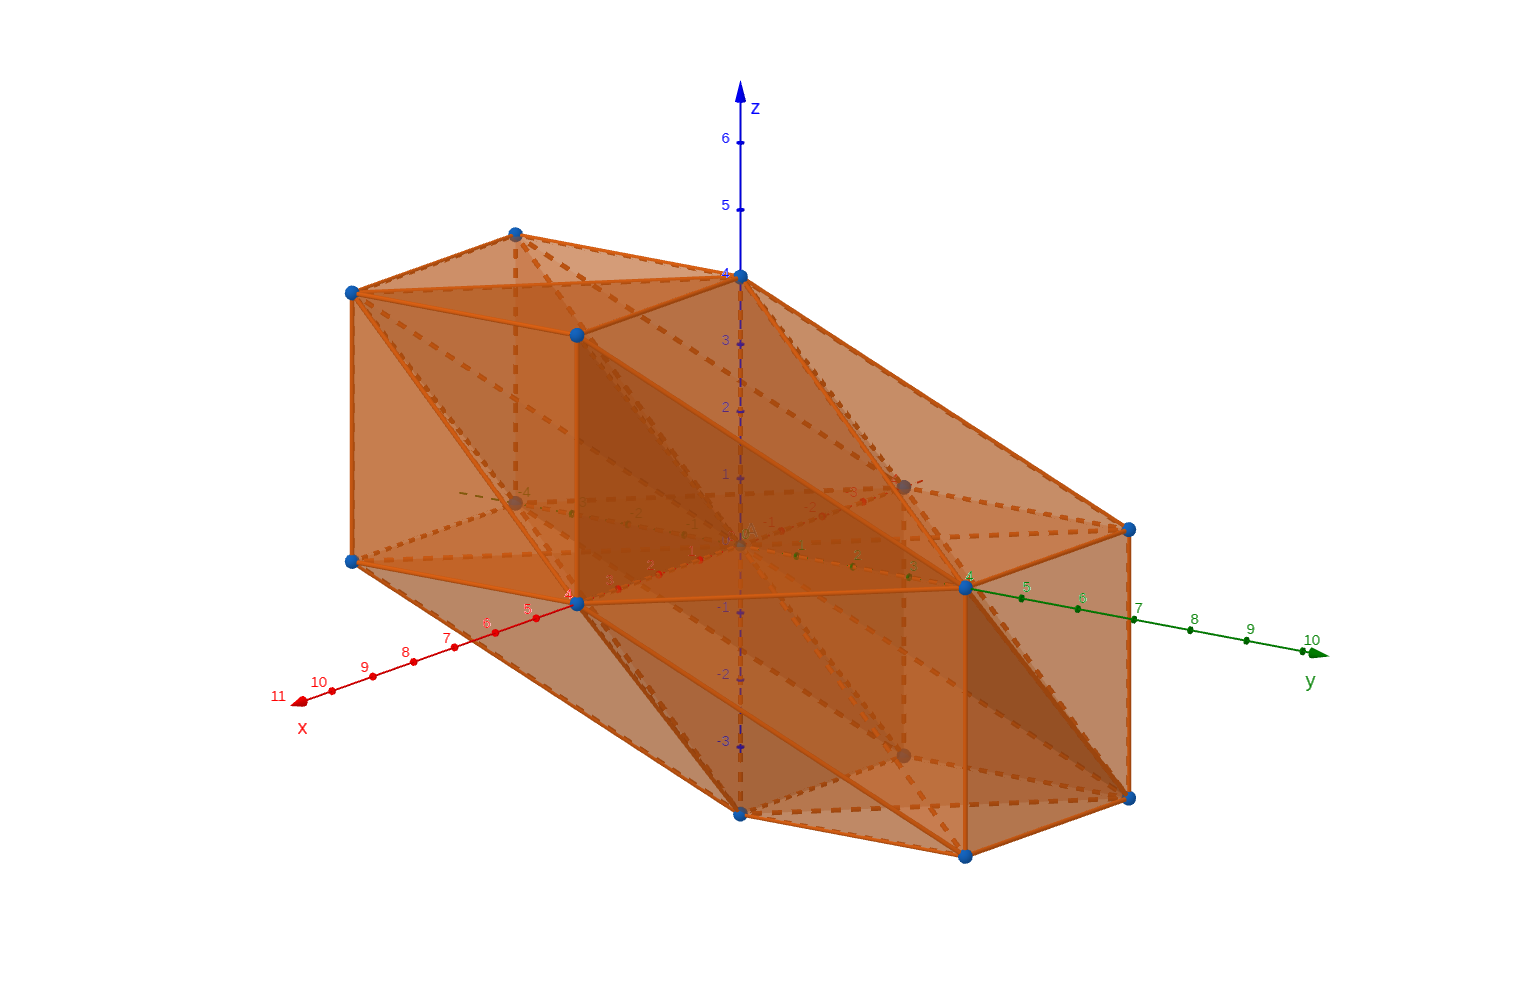
\includegraphics[width=\textwidth]{./pics/final/adjacent.png}  
        \caption{Neighbour nodes of center}  
        \label{fig:sub2} 
    \end{subfigure}%  
    \begin{subfigure}{0.5\textwidth}  
        \centering  
        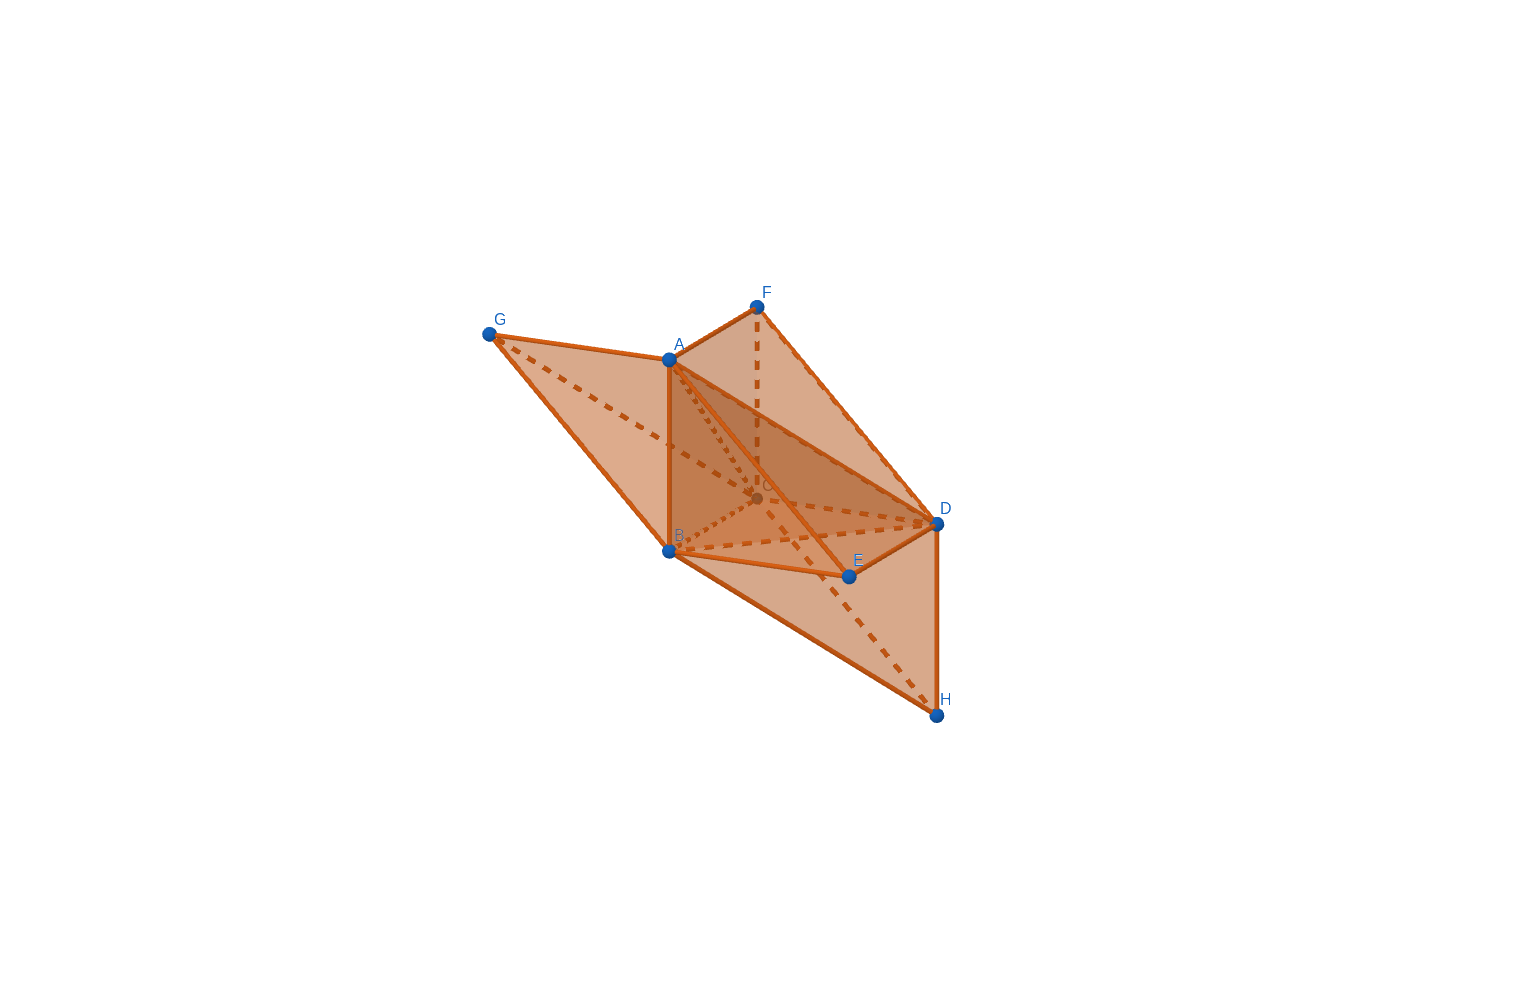
\includegraphics[width=\textwidth]{./pics/final/3D.png}  
        \caption{Cells to Nodes}  
    \end{subfigure} 
\end{figure}
并且我们可以发现,在DG方法中定义的跳量以及平均都可以储存在边上。我们也可以发现,在DG方法中,我们装配的刚度矩阵和图神经网络中的邻接矩阵有很多的共同点,并且已经有工作涉及DG方法和GNN融合,但还是聚焦在如何求解刚度矩阵的线性方程组。

%   \begin{figure}[H]
%     \centering
%     \begin{tikzpicture}
%         % 输入层
%         \draw (0, 4) circle [radius=0.3];
%         \node (I1)at (0,4) {1};

%         \draw (0, 6) circle [radius=0.3];
%         \node (I2)at (0,6) {2};
        
%         % 隐藏层
%         \foreach \i in {1,...,10} {
%             \draw (3, \i) circle [radius=0.3];
%             \node (H1\i)at (3,\i) {};
%         }

%         \foreach \i in {1,...,10} {
%             \draw (6, \i) circle [radius=0.3];
%             \node (H2\i)at (6,\i) {};
%         }
        
%         % 输出层
%         \foreach \i in {1} {
%             \node (O\i)at (9,5) {$u(x,y,t)$};
%         }
        
%         % 连接输入层和隐藏层
%         \foreach \i in {1,2} {
%             \foreach \j in {1,...,10} {
%                 \draw[->] (I\i) -- (H1\j);
%             }
%         }
%         \foreach \i in {1,...,10} {
%             \foreach \j in {1,...,10} {
%                 \draw[->] (H1\i) -- (H2\j);
%             }
%         }
        
%         % 连接隐藏层和输出层
%         \foreach \i in {1,...,10} {
%             \draw[->] (H2\i) -- (O1);
%         }
%     \end{tikzpicture}
%     \caption*{MLP for basis function $Net_i$ for $Cid_i$}    
% \end{figure}

